\section{Behaviors}
\label{sec:Behaviors}
% Owner: 
% Reviewed:
%
The addressed solution provides in its default setting already several behaviors for merchants as well as the consumers. The former include known rule-based strategies like the ``Gas Station strategy'', ``Be the n-cheapest'', ``fix price'' as well as a first data-driven approach implementing logistic regression \citep{hosmer2013applied}.
%
\begin{figure}[h]
    \centering
    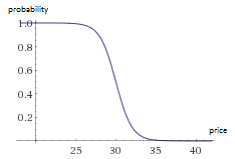
\includegraphics[width=0.5\textwidth]{images/sigmoid.png}
    \caption{Sigmoid distribution as consumer behavior}
    \label{fig:sigmoid_distribution}
\end{figure}
%
Additionally, a consumer is included implementing several buying behaviors which can be chosen, weighted and altered on-the-fly. Those behaviors range from very subtle approaches like buying the n-cheapest, first, most expensive or simple random up to more sophisticated methods trying to imitate more complex consumer situations. A sigmoid distribution with twice of the producer price as mean (see fig. \ref{fig:sigmoid_distribution}) is available through the default settings as well as a logistic regression evaluation of provided coefficients which are used to calculate selling probability for consumer to buy.

%
\begin{figure}[h]
    \centering
    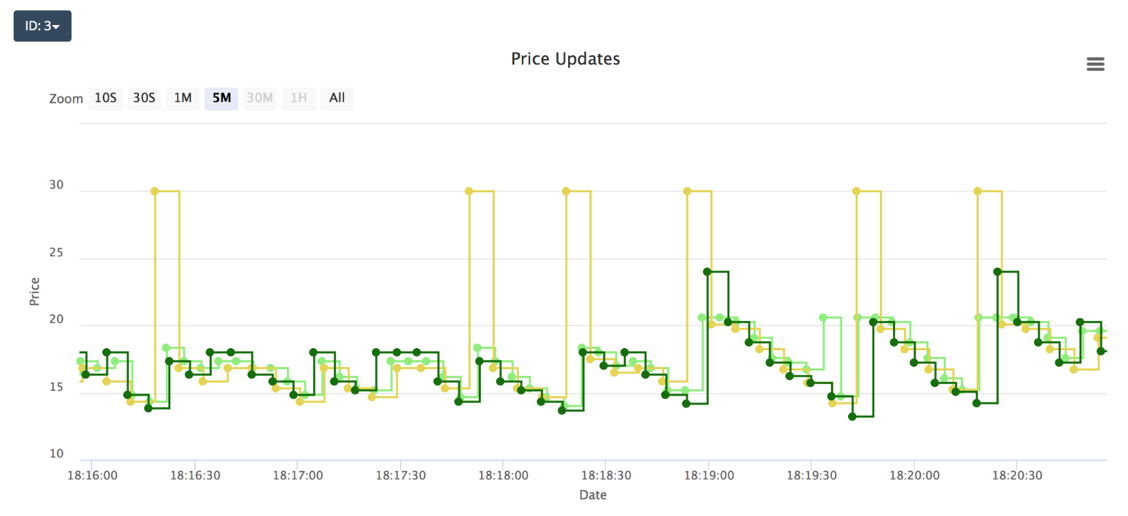
\includegraphics[width=0.5\textwidth]{images/price_graphs_v2.png}
    \caption{Price Graphs}
    \label{fig:price_graphs_v2}
\end{figure}
%